\documentclass{article}
% Pacchetti di Codifica e Lingua
\usepackage[utf8]{inputenc}
\usepackage[T1]{fontenc}
\usepackage[italian]{babel}

% Pacchetti Grafici e Diagrammi
\usepackage{graphicx}
\usepackage{tikz}
\usepackage{circuitikz}
\usepackage{tikz-3dplot}
\usetikzlibrary{angles,quotes,arrows.meta, positioning}
\usepackage{pgfplots}
\pgfplotsset{compat=1.18}

% Pacchetti Matematici
\usepackage{amsmath, amssymb, amsthm}

% Pacchetti per Tabelle e Unità di Misura
\usepackage{geometry}
\usepackage{siunitx}
\usepackage{booktabs}
\usepackage{tabularx}
\usepackage{colortbl}
\usepackage{adjustbox}

% Pacchetti per Layout e Formattazione
\usepackage{fancyhdr}
\usepackage{float}
\usepackage{microtype}

% Altri Pacchetti Utili
\usepackage{mdframed}
\usepackage{animate}
\usepackage{ulem}
\usepackage{eurosym}

% Pacchetto enumitem
\usepackage{enumitem}

% Definizioni dei Colori
\definecolor{lightblue}{HTML}{9cd8fc}
\definecolor{myblue}{HTML}{139FE9}
\definecolor{myblack}{HTML}{303030}
\definecolor{mygray}{HTML}{787878}
\definecolor{mywhite}{HTML}{c7c7c7}

%\pagecolor{myblack}
%\color{mywhite}
% Definizione del comando \norm
\newcommand{\norm}[1]{\left\lVert#1\right\rVert}

%\font\nullfont=cmr10 

% Ambienti Personalizzati
\newmdtheoremenv[
    backgroundcolor=orange!10,
    linecolor=myblue,
    linewidth=0pt,
    leftmargin=0pt,
    rightmargin=0pt,
    innerleftmargin=10pt,
    innerrightmargin=10pt,
    innertopmargin=10pt,
    innerbottommargin=10pt,
    nobreak
]{curiosity}{Curiosità}

\newmdtheoremenv[
    font=\normalfont\small,
    linewidth=0pt,
    innerleftmargin=10pt,
    innerrightmargin=10pt,
]{example}{Esempio}

\newmdtheoremenv[
  backgroundcolor=lightblue,
  linecolor=myblue,
  linewidth=1.5pt,
  innertopmargin=10pt,
  innerbottommargin=10pt,
  innerrightmargin=10pt,
  innerleftmargin=10pt,
  nobreak
]{theorem}{Teorema}

\newmdtheoremenv[
  backgroundcolor=gray!10,
  linewidth=0pt,
  innertopmargin=10pt,
  innerbottommargin=10pt,
  innerrightmargin=10pt,
  innerleftmargin=10pt,
  nobreak
]{definition}{Definizione}

\newmdtheoremenv[
  backgroundcolor=gray!10,
  linecolor=myblue,
  linewidth=1.5pt,
  innertopmargin=10pt,
  innerbottommargin=10pt,
  innerrightmargin=10pt,
  innerleftmargin=10pt,
  nobreak
]{proposition}{Proposizione}

% Configurazioni di fancyhdr
\pagestyle{fancy}
\fancyhf{} % Pulisce tutti i campi
\fancyhead[LO]{\nouppercase{\rightmark}} % Titolo della sezione
\renewcommand{\headrulewidth}{0.5pt}
\renewcommand{\footrulewidth}{0pt}

\geometry{a4paper, left=20mm, right=20mm, top=20mm, bottom=20mm}

% Pacchetto Hyperref (inserito per ultimo)
\usepackage{hyperref}
% Additional Packages
\usepackage{xparse,array}

\begin{document}
\begin{titlepage}
    \centering
    \vspace*{1cm} % Aggiunge spazio verticale
    
\includegraphics[width=0.6\textwidth]{src/logo.png} % Inserisci il percorso corretto al file del logo
    \vspace{1.5cm}
    
    \Huge
    \textbf{Informe de Laboratorio de Electrotécnia}
    
    \vspace{0.5cm}
    \LARGE
    Práctica 2
    
    \vspace{1.5cm}
    
    \textbf{Michele Mazza y Juan Repiso}
    
    \vfill
    
    \Large
    Grado en Ingeniería de Sistemas Industriales\\
    Universidad Alfonso X el Sabio\\
    \today
\end{titlepage}
\section{Introducción}
En el informe de Laboratorio dado, se describe la investigación realizada en el laboratorio de Electrotécnia de dos circuitos de corriente alterna con enfoque en el factor de potencia relacionado a circuitos en serie y paralelo. El objetivo sería de manipular los valores de los componentes para obtener un factor de potencia, \textbf{f.d.p}, $\cos(\varphi) \geq 0.95$. Primero medimos los valores de la resistencia que se utilizarà.
\begin{itemize}
  \item $R = 158 \Omega$ 
\end{itemize}
\section{Procedimiento Experimental}

\begin{enumerate}
    \item \textbf{Ajuste de las Perillas de $L$ y $C$}
    \begin{itemize}
        \item Utilizar las perillas de los instrumentos para seleccionar una posición inicial del inductor $(L)$ y del condensador $(C)$, estableciendo valores que determinen respectivamente una carga inductiva y una carga capacitiva.
    \end{itemize}

    \item \textbf{Montaje del Circuito sin Tensión}
    \begin{itemize}
        \item Montar el circuito sin aplicar tensión, conectando en serie los siguientes componentes:
        \begin{itemize}
            \item Generador de tensión alterna $(V_{\text{fuente}})$.
            \item Amperímetro para medir la corriente total $(I_{\text{total}})$.
            \item Resistencia $(R)$.
            \item Inductor $(L)$.
            \item Condensador $(C)$.
        \end{itemize}
        \item Una vez completado el montaje, informar al profesor para que verifique el circuito antes de energizarlo.
    \end{itemize}

    \item \textbf{Medición de $V_{\text{fuente}}$ e $I_{\text{total}}$, Cálculo de $Z$ y $\varphi$}
    \begin{itemize}
        \item Energizar el circuito y medir:
        \begin{itemize}
            \item La tensión de alimentación $V_{\text{fuente}}$.
            \item La corriente total $I_{\text{total}}$.
        \end{itemize}
        \item Calcular la impedancia total $Z$ del circuito:
        \[
        Z = \frac{V_{\text{fuente}}}{I_{\text{total}}}
        \]
        \item Determinar el ángulo de fase $\varphi$ entre la tensión y la corriente:
        \[
        \cos \varphi
        \]
        \item \textbf{Evaluación del Factor de Potencia:}
        \begin{itemize}
            \item Si $\cos \varphi < 0{,}95$, volver al \textbf{Paso 1} y ajustar nuevamente los valores de $L$ y $C$.
            \item Si $\cos \varphi \geq 0{,}95$, proceder al \textbf{Paso 4}.
        \end{itemize}
    \end{itemize}

    \item \textbf{Medición de las Caídas de Tensión en $V_L$ y $V_C$}
    \begin{itemize}
        \item Medir las tensiones al lado del inductor $(V_L)$ y del condensador $(V_C)$ utilizando voltímetros adecuados.
    \end{itemize}

    \item \textbf{Cálculo de las Reactancias $X_L$ y $X_C$, Determinación de $L$ y $C$}
    \begin{itemize}
        \item Calcular las reactancias inductiva $(X_L)$ y capacitiva $(X_C)$:

        \item Determinar los valores efectivos de $L$ y $C$:
        \[
        L = \frac{X_L}{2\pi f}
        \]
        \[
        C = \frac{1}{2\pi f X_C}
        \]
        \item Donde $f$ es la frecuencia de la fuente de tensión alterna.
    \end{itemize}

    \item \textbf{Cálculo de las Potencias $S$, $P$ y $Q$}
    \begin{itemize}
        \item Calcular la potencia aparente $(S)$:
        \[
        S = V_{\text{fuente}} \times I_{\text{total}}
        \]
        \item Calcular la potencia activa $(P)$ y la potencia reactiva $(Q)$:
        \[
        P = S \times \cos \varphi
        \]
        \[
        Q = S \times \sin \varphi
        \]
    \end{itemize}

    \item \textbf{Representaciones Gráficas}
    \begin{itemize}
        \item \textbf{Diagrama Fasorial:}
        \begin{itemize}
            \item Dibujar el diagrama fasorial de las tensiones y corrientes, indicando los fasores de $V_{\text{fuente}}$, $I_{\text{total}}$
        \end{itemize}
        \item \textbf{Triángulo de Potencias:}
        \begin{itemize}
            \item Representar gráficamente el triángulo de potencias, mostrando la relación entre $P$, $Q$ y $S$.
        \end{itemize}
        \item \textbf{Gráfico de las Ondas de Tensión y Corriente:}
        \begin{itemize}
            \item Trazar los gráficos de las formas de onda de la tensión $v(t)$ y la corriente $i(t)$ en el dominio del tiempo, resaltando el desfase $\varphi$ entre ellas.
        \end{itemize}
    \end{itemize}

\end{enumerate}
\section{Montaje 1}
En este experimento de laboratorio, analizamos un circuito RLC en serie alimentado con corriente alterna, con el objetivo de optimizar el factor de potencia  $(\cos \varphi)$  acercándolo lo más posible al valor de $0,95$. Para lograr esto, variamos las configuraciones del inductor  $(L)$  y del condensador  $(C)$  utilizando sus respectivas perillas de ajuste. La mejora del factor de potencia es fundamental en aplicaciones prácticas para aumentar la eficiencia energética y reducir las pérdidas en el sistema eléctrico.
\begin{figure}[H]
  \centering
  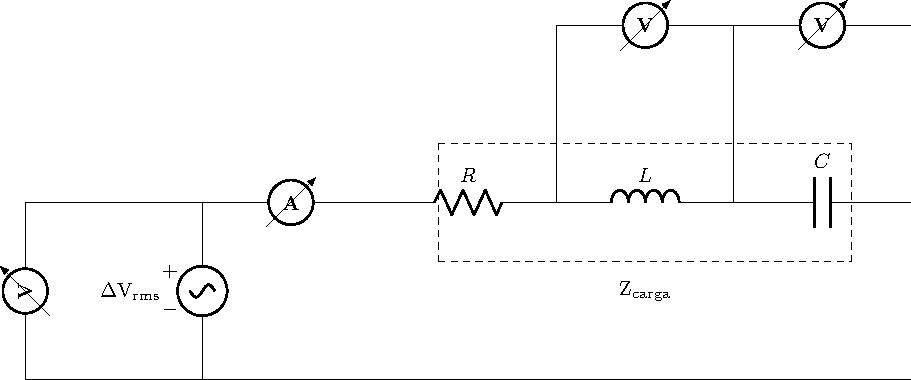
\includegraphics{src/circuit01.pdf}
  \caption{Circuito 1}
  \label{fig:circuit01}
\end{figure}
\subsection{Procedimiento}
\begin{enumerate}
  \item Después de diferentes ajustes y medidas hemos obtenido los siguientes resultados ajustando las perillas de $L$ oltre la midad y $C$ a poco meno de la mitad.
  \item El circuito fuè revisado
  \item Los valores obtenidos son:
  \begin{itemize}
    \item Tensión de alimentación medida $V_{\text{fuente}} = 146 \si{\volt}$
    \item Corriente total medida $I_{\text{total}} = 0.878 \si{\ampere}$
    \item Impedancia total 
    \[
    Z = \frac{V_{\text{fuente}}}{I_{\text{total}}} = \frac{146}{0.878} = 166.25 \si{\ohm}
    \]
    \item Evaluación del factor de potencia
    \[
    \cos \varphi = \frac{R}{Z} = \frac{158}{166.25} = 0.951
    \]
    \[
    \varphi = \arccos(0.951) = 18.01 \si{\degree}
    \]
    dado que $\cos \varphi \geq 0.95$ procedemos al paso 4.
  \end{itemize}
  \item Medición de las caídas de tensión en $V_L$ y $V_C$
  \begin{itemize}
    \item $V_L = 82.8 \si{\volt}$
    \item $V_C = 37.5 \si{\volt}$
  \end{itemize}
  \item Cálculo de las reactancias $X_L$ y $X_C$, determinación de $L$ y $C$
  \begin{itemize}
    \item Reactancia inductiva
    \[
    X_L = \frac{V_L}{I_{\text{total}}} = \frac{82.8 \si{\volt}}{0.878\si{\ampere}} = 94.3 \si{\ohm}
    \]
    \item Reactancia capacitiva
    \[
    X_C = \frac{V_C}{I_{\text{total}}} = \frac{37.5\si{\volt}}{0.878\si{\ampere}} = 42.7 \si{\ohm}
    \]
    \item Valores efectivos de $L$ y $C$
    \[
    L = \frac{X_L}{2\pi f} = \frac{94.3\si{\ohm}}{2\pi \cdot 50\si{\hertz}} = 0.3 \si{\henry}
    \]
    \[
    C = \frac{1}{2\pi f X_C} = \frac{1}{2\pi \cdot 50 \si{\hertz} \cdot 42.7\si{\ohm}} = 74 \si{\micro\farad}
    \]
  \end{itemize}
  \item Cálculo de las potencias $S$, $P$ y $Q$
  \begin{itemize}
    \item Potencia aparente
    \[
    S = V_{\text{fuente}} \times I_{\text{total}} = 146 \si{\volt} \times 0.878 \si{\ampere} = 128 \si{\volt\ampere}
    \]
    \item Potencia activa
    \[
    P = S \times \cos \varphi = 128 \si{\volt\ampere} \times 0.951 = 121.6 \si{\watt}
    \]
    \item Potencia reactiva
    \[
    Q = S \times \sin \varphi = 128 \si{\volt\ampere} \times \sin(18.01\si{\degree}) = 39.6 \mathrm{VAr}
    \]
  \end{itemize}
  \item Representaciones gráficas
  \begin{itemize}
    \item Diagrama fasorial
    \begin{figure}[H]
      \centering
      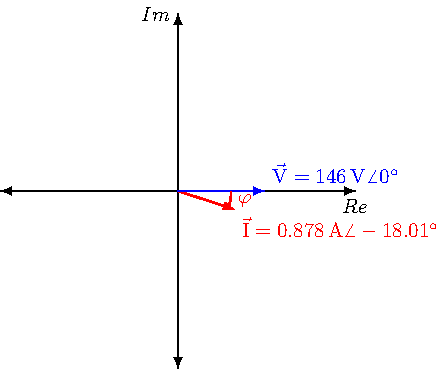
\includegraphics{src/fasorial01.pdf}
      \caption{Diagramas Fasoriales}
      \label{fig:fasorial01}
    \end{figure}
    \item Triángulo de Potencias
    \begin{figure}[H]
      \centering
      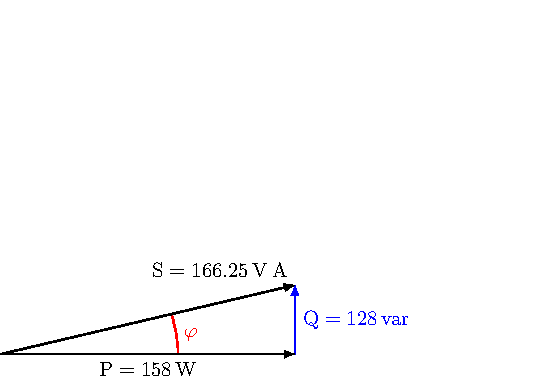
\includegraphics{src/triangulo01.pdf}
      \caption{Triángulo de Potencias}
      \label{fig:potencias01}
    \end{figure}
    \item Gráfico de las Ondas de Tensión y Corriente
    \begin{figure}[H]
      \centering
      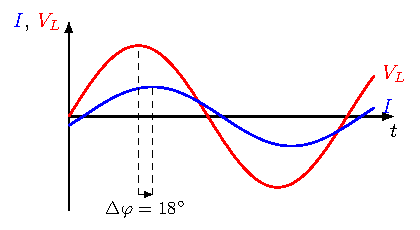
\includegraphics{src/ondas01.pdf}
      \caption{Gráficos de las Ondas de Tensión y Corriente}
      \label{fig:ondas01}
    \end{figure}
  \end{itemize} 
\end{enumerate}
\section{Montaje 2}

En este experimento, analizamos un circuito RLC en paralelo alimentado con corriente alterna, con el objetivo de estudiar el factor de potencia en un circuito en paralelo y comprender por qué no se alcanza un valor óptimo de $\cos \varphi$.

\begin{figure}[H]
\centering
  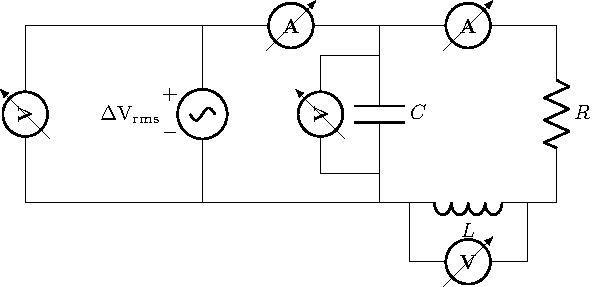
\includegraphics{src/circuit02.pdf}
  \caption{Circuito 2}
  \label{fig:circuit02}
\end{figure}

\subsection{Procedimiento}
\begin{enumerate}
  \item Después de diferentes ajustes y medidas, se realizó el montaje del circuito en paralelo, se logró obtener un $\cos \varphi$ óptimo.
  \item El circuito fue revisado por el profesor para verificar su correcta configuración.
  \item Los valores obtenidos son:
  \begin{itemize}
    \item Tensión de alimentación medida: $V_{\text{fuente}} = 99.06\,\si{\volt}$, frecuencia $f = 50\,\si{\hertz}$
    \item Corriente total medida: $I_{\text{total}} = 0.36 \,\si{\ampere}$
    \item Resistencia: $R = 240\,\si{\ohm}$
    \item Corriente en la rama con $R$ y $L$: $I_{\text{RL}} = 0.38\,\si{\ampere}$
    \item Corriente en la rama con el Condensador: $I_{\text{C}} = 0.06\,\si{\ampere}$
    \item Tensión en el inductor: $V_L = 38 \,\si{\volt}$
    \item Tensión en el condensador: $V_C = 99.06\,\si{\volt}$
  \end{itemize}
  \subsubsection{Cálculo de las Reactancias y Comprobación del Factor de Potencia}
\end{enumerate}
\begin{enumerate}
    \item \textbf{Cálculo de la Reactancia Inductiva $X_L$ y del Valor de $L$}

    Dado que la tensión medida en el inductor es $V_L = 38\,\si{\volt}$ y la corriente que atraviesa la rama R--L es 
    $I_{\text{RL}} = 0.38\,\si{\ampere}$, podemos calcular la reactancia inductiva:

    \[
    X_L = \frac{V_L}{I_{\text{RL}}} 
         = \frac{38\,\si{\volt}}{0.38\,\si{\ampere}}
         \approx 100\,\Omega.
    \]

    Conociendo la frecuencia de la fuente ($f=50\,\si{\hertz}$) y 
    $\omega = 2\pi f = 314.16\,\si{\radian/\second}$, el valor de la inductancia es:

    \[
    L = \frac{X_L}{\omega}
       = \frac{100\,\Omega}{314.16\,\si{\radian/\second}}
       \approx 0.32\,\si{\henry}.
    \]

    \item \textbf{Cálculo de la Reactancia Capacitiva $X_C$ y del Valor de $C$}

    El condensador está en paralelo a la misma tensión de alimentación 
    $V_C = 99.06\,\si{\volt}$ (ya que es un circuito en paralelo), y la corriente que lo atraviesa es $I_C \approx 0.06\,\si{\ampere}$.  
    Por tanto, su reactancia capacitiva es:

    \[
    X_C = \frac{V_C}{I_C} 
         = \frac{99.06\,\si{\volt}}{0.06\,\si{\ampere}}
         \approx 1651\,\Omega.
    \]

    Así, el valor de la capacidad se obtiene de:

    \[
    C = \frac{1}{\omega\,X_C}
       = \frac{1}{314.16 \times 1651}
       \approx 1.94\times 10^{-6}\,\si{\farad}
       = 1.94\,\si{\micro\farad}.
    \]

    \item \textbf{Factor de Potencia del Circuito en Paralelo}

    Se midió una corriente total de $I_{\text{total}} = 0.36\,\si{\ampere}$, 
    con una tensión en bornes de $V_{\text{fuente}} = 99.06\,\si{\volt}$.  
    A partir de mediciones o del diagrama fasorial, se ha obtenido 
    un ángulo de desfase $\varphi \approx -14.6^\circ$ (circuito ligeramente inductivo).  
    El factor de potencia resulta:

    \[
    \cos\varphi \approx \cos(-14.6^\circ) \approx 0.97.
    \]

    \item \textbf{Cálculo de las Potencias $S$, $P$ y $Q$}

    \begin{itemize}
        \item \textbf{Potencia aparente, $S$}:  
        \[
        S = V_{\text{fuente}} \cdot I_{\text{total}}
          = 99.06\,\si{\volt} \times 0.36\,\si{\ampere}
          \approx 35.66\,\si{\volt\ampere}.
        \]

        \item \textbf{Potencia activa, $P$}:  
        \[
        P = S \times \cos \varphi
          \approx 35.66 \,\si{\volt\ampere} \times 0.97
          \approx 34.59\,\si{\watt}.
        \]

        \item \textbf{Potencia reactiva, $Q$}:  
        \[
        Q = S \times \sin \varphi
          \approx 35.66 \,\si{\volt\ampere} \times \sin(14.6^\circ)
          \approx 9.0\,\mathrm{VAr}.
        \]
    \end{itemize}
    \item Representaciones gráficas:
  \begin{itemize}
    \item Diagrama fasorial:
    \begin{figure}[H]
      \centering
      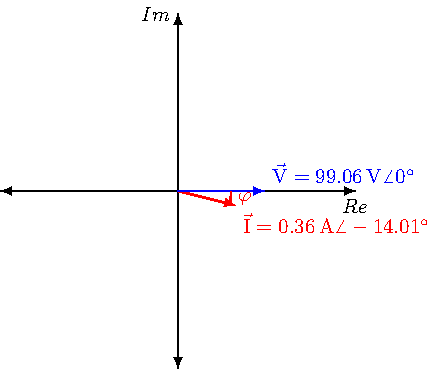
\includegraphics{src/fasorial02.pdf}
      \caption{Diagrama Fasorial del Montaje 2}
      \label{fig:fasorial02}
    \end{figure}
    \item Triángulo de potencias:
    \begin{figure}[H]
      \centering
      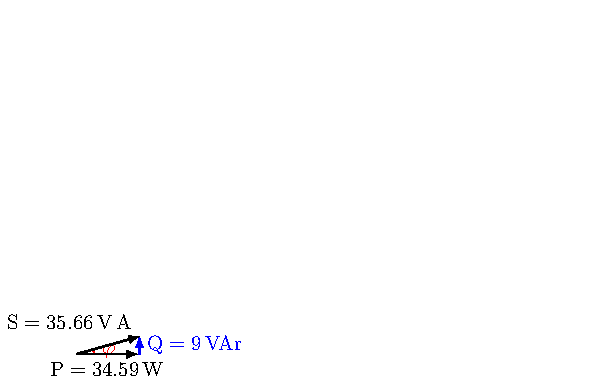
\includegraphics{src/triangulo02.pdf}
      \caption{Triángulo de Potencias del Montaje 2}
      \label{fig:potencias02}
    \end{figure}
    \item Gráfico de las ondas de tensión y corriente:
    \begin{figure}[H]
      \centering
      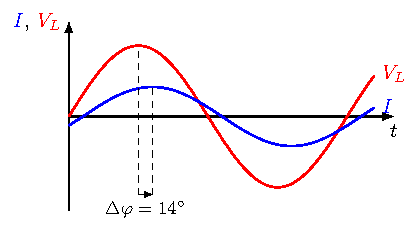
\includegraphics{src/ondas02.pdf}
      \caption{Gráficos de las Ondas de Tensión y Corriente}
      \label{fig:ondas02}
    \end{figure}
  \end{itemize}

\end{enumerate}
  
\end{document}